\chapter{Implementação}\label{chap:chap4}

% \section*{}
% Este capítulo pode ser dedicado à apresentação de detalhes de nível
% mais baixo relacionados com o enquadramento e implementação das
% soluções preconizadas no capítulo anterior.
% Note-se no entanto que detalhes desnecessários à compreensão do
% trabalho devem ser remetidos para anexos.

% Dependendo do volume, a avaliação do trabalho pode ser incluída neste
% capítulo ou pode constituir um capítulo separado.

A ideia principal do projeto seria fazer a deteção de objetos simples e depois capitalizar nessa capacidade desenvolvida para fazer a deteção de objetos mais complexos. Esta deteção de objetos, que culminou na escolha da mesa como caso de estudo pelas considerações que já foram explanadas da sua morfologia, tem commo objetivo último a sua utilização num demonstrador de robótica autónoma, fazendo recurso a um dicionário pré-existente em que as mesas conhecidas são listadas num ficheiro \emph{XML}.

O programa desenvolvido foi escrito em \emph{C++} recorrendo a algumas bibliotecas informáticas, nomeadamente a \emph{Point Cloud Library} (PCL) para a captura e manipulação de nuvens de pontos, \emph{Boost}. De seguida são analisados com mais detalhe os pormenores de implementação.

\section{Captura de Imagens 3D para análise }

A captura de imagens em 3D foi desenvolvida utilizando o a biblioteca \emph{Point Cloud Library}, e é uma das opções do projeto associado a esta dissertação. As nuvens de pontos são guardadas em ficheiros PCD e guardam o que é capturado pelo \emph{Kinect}, sendo que contém toda a informação RGBD e pode ser visualizada com a mesma aplicação que as gerou.

\begin{center}
	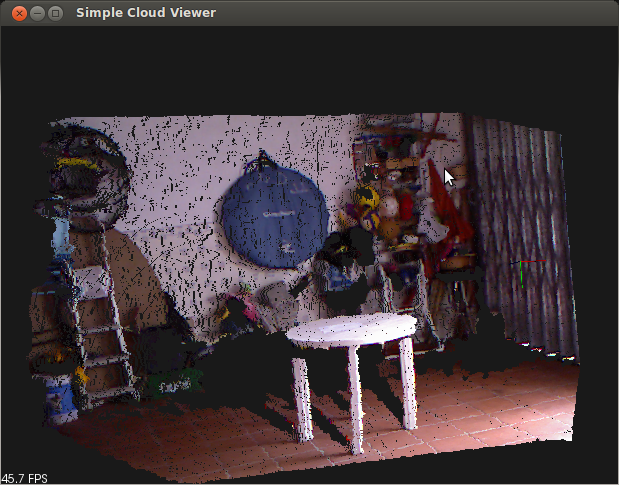
\includegraphics[width=0.80\textwidth]{figures/exemplo_captura.png}
	\captionof{figure}{Exemplo de imagem capturada com informação RGBD onde se pesquisará mesas.}
	\label{fig:exemplo_captura}
\end{center}

\subsection{Análise seleção e Separação de amostra de controlo}

Selecionou-se imagens com mesas para testar a qualidade de deteção após o desenvolvimento da tese, para avaliar a adequação da solução ao problema.

\section {Implementação da Deteção}

Agora serão listados todos os passos por que passa uma imagem RGBD para se poder detetar a existência de mesas na nuvem de pontos.

Antes de tudo a informação RGB é descartada pois não tem uma grande influência sobre deteção, isto porque após considerações cuidadosas chegou-se à conclusão que a cor não é um aspeto que tenha grande peso na caracterização da mesa.


Adicionalmente o dicionário de mesas conhecidas é lido a partir do ficheiro \emph{dictionary.xml} e guardado em memória para se poder fazer a comparação com o que é encontrado na imagem e dar um valor que avalia a confiança com que pode garantira que é a mesa indicada.

Um exemplo de como é descrita uma mesa em XML:
\begin{verbatim}
	<table>
	<name>Mesa 1</name>
	<top shape="circular" large_dimension="0.89" small_dimension="0.89"/>
	<legs  number="4" height="0.68" parallel="true" center_distance="0.8"/>
	</table>
\end{verbatim}
As características das mesas são distribuídas entre o tampo da mesa e as pernas, descrevendo a sua morfologia em tanto parâmetros quantitativos como a altura e dimensões dos tampos como em parâmetros qualitativos como a geometria do tampo e se as pernas são paralelas.

\subsection{Pré Processamento}

Agora que se trabalha sobre a informação de profundidade, que se encontra em SI (metros), é feito um pré processamento onde se descarta tudo que aparece na imagem que dista a mais de 4,5 metros do sensor. Isto é no sentido de eliminar erros persistentes na imagem, pois o \emp{Kinect} vai perdendo precisão com a distância\footnote{fundamentar isto}. No passo seguinte vai-se remover o maior plano que corresponde ao chão, de modo a isolar os objetos que se encontrem na imagem.


Depois é feita uma clusterização usando o algoritmo k-d Tree para separar o que resta da imagem em objetos coerentes e separáveis. Isto, dando um exemplo prático, é para não acontecer o caso de estarmos a reconhecer o que parece uma perna de uma mesa a dois metros de distância do que é reconhecido como um tampo.

No final deste pré processamento o resultado será um conjunto de nuvens de pontos, em que cada uma representa um objeto que se encontra na imagem capturada inicial.


\begin{center}
	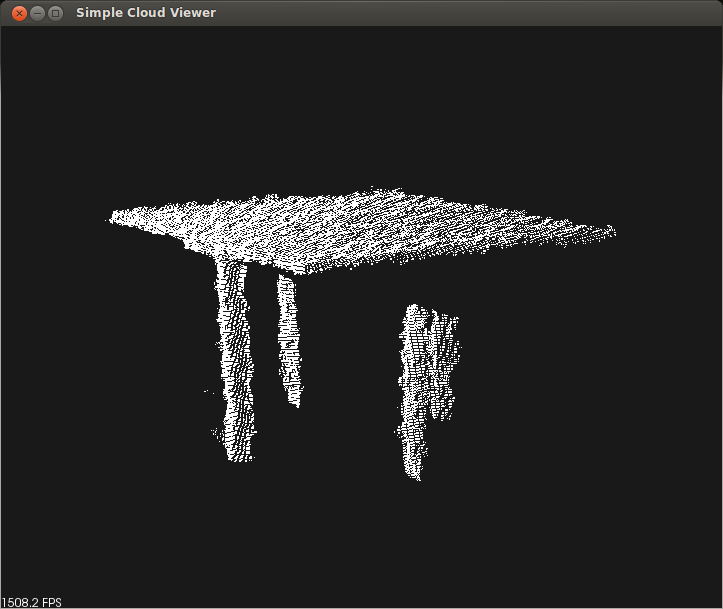
\includegraphics[width=0.80\textwidth]{figures/exemplo_mesa2.png}
	\captionof{figure}{Exemplo de imagem após pré processamento.}
	\label{fig:exemplo_processado}
\end{center}


\subsection{Deteção de Mesas}

De seguida cada um dos objetos separados passa por um processo onde se tenta 
detetar constituintes das mesas, como pernas e tampos. Caso sejam encontrados 
verifica-se se correspondem a alguma das mesas conhecidas que estão guardadas
no dicionário das mesas conhecidas.

Esta deteção é feita nos seguintes passos: primeiro faz-se a deteção do tampo, que é obrigatoriamente uma superfície planar, e caso não tenha um plano é logo atribuída uma confiança de 0, considerando-se que não é uma mesa.
Caso exista um plano, as suas dimensões são avaliadas e comparadas com cada um dos modelos.

% explicar a fórmula de comparação

Com base no que foi detetado, utilizando uma metodologia fuzzy, foram combinados os fatores de confiança na deteção dos objetos simples para dar um fator de confiança de ser alguma das mesas já conhecidas.

% Contudo essa ideia foi simplificada aquando da implementação, pois a PCL permite já fazer a deteção de algumas dessas primitivas mas principalmente porque o processo de identificação é muito custoso em termos de tempo de execução, atrasando o reconhecimento e não trazendo r


\section {Resultados Obtidos}

TBD

\section{Resumo}


